\chapterimage{chapterimage_1.jpg} % Chapter heading image

\chapter{Overview of the \ate{} UI}
\section{Introduction}\index{Introduction}

\doublespacing
This chapter gives an overview of the software that is named \emph{ATExplorer}.

The following section discusses the application in greater detail.

\clearpage

\section{The \ate UI}

\begin{figure}[h]
\centering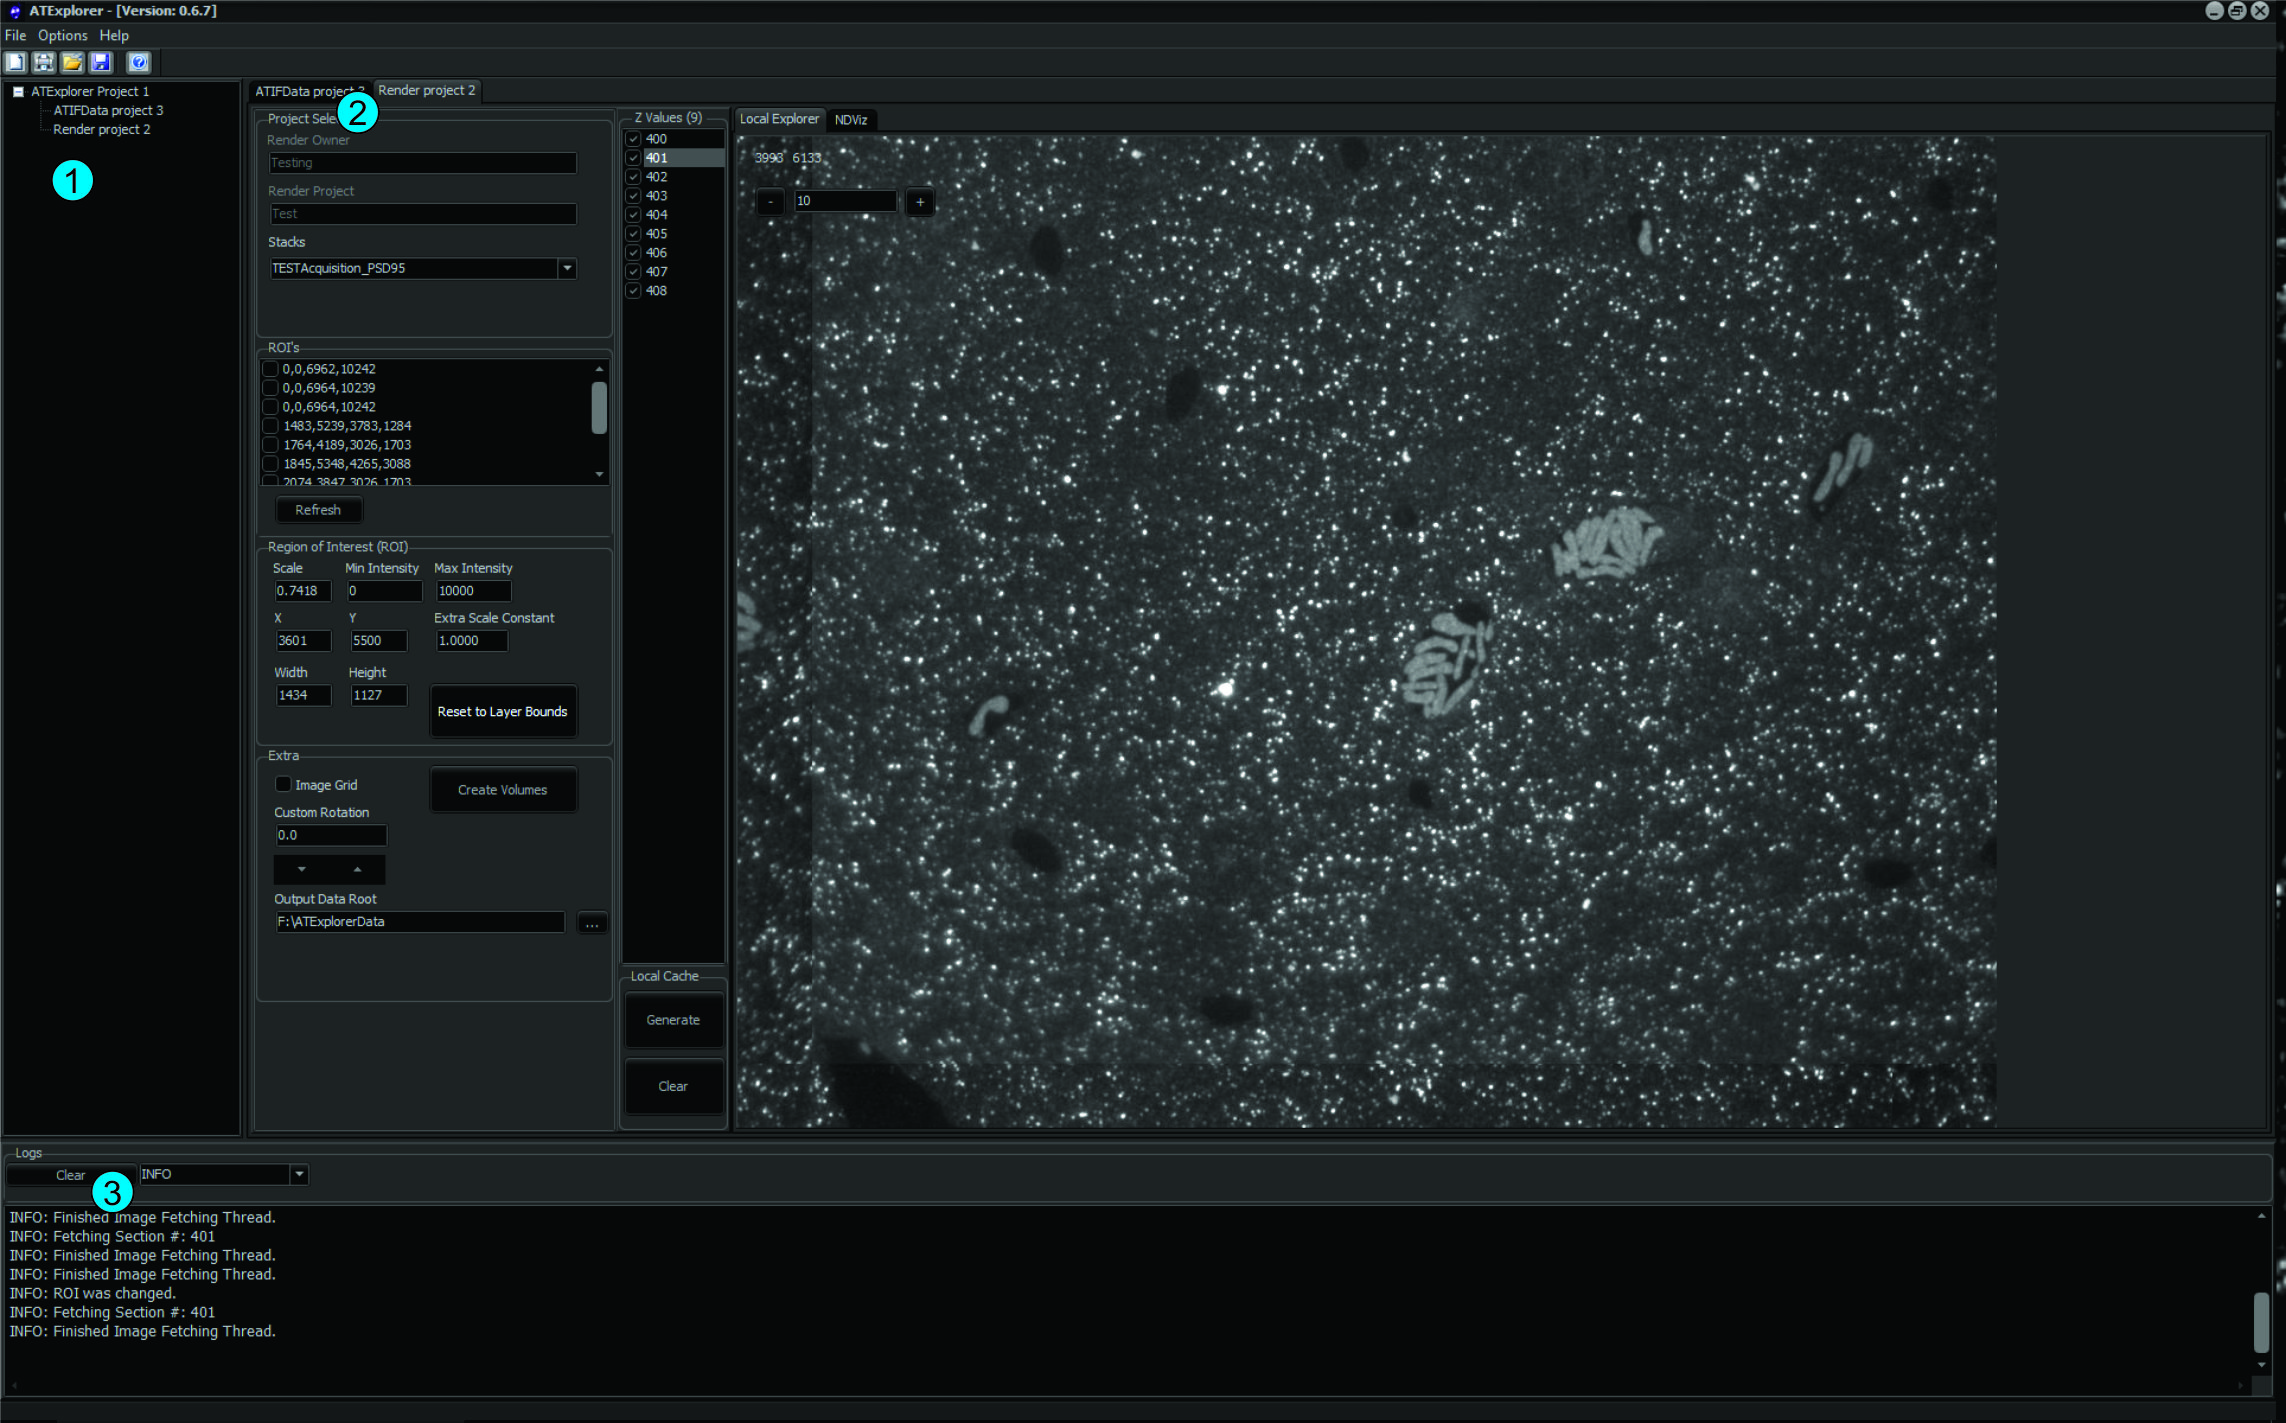
\includegraphics[scale=0.85]{ATExplorerUI_1}

\caption{\ate{} UI. The circled numbers in the figure indicate relevant elements of the UI; \protect\cn{1} Project(s) TreeView. \protect\cn{2} Tabbed Project Item View. \protect\cn{3} Information and Application Log Messages.}
\end{figure}

\subsection{Importing Data}

\begin{description}[font=$\bullet$~\normalfont\scshape\color{red!50!black}]
\item [Importing process] Give an overview on what happens when data is being imported to \ate.
\item [Data Formats] Mention the Allen Institute format, and Kristinas format.
\end{description}

\subsection{Processing Data}
\begin{description}[font=$\bullet$~\normalfont\scshape\color{red!50!black}]
\item [FlatField correction]
\item [Rough aligning] 
\item [Fine aligning] 
\item [Other]
\end{description}

\subsection{Connecting to a a Remote (or local) RenderHost}

\subsection{Managing Stacks in Render}

\subsection{Exploring Data}


\clearpage

